% VetNutri MP user guide — desktop version (English translation of guide_utilisateur.tex)
% Build: latexmk -pdf user_guide_en.tex
% Screenshots (captures/) are shared with the French guide and show the French interface;
% see README.md. Numbered markers are placed in screenshot pixels (1400 x 900): \repere{x}{y}{n}.

\documentclass[11pt,a4paper]{article}

\usepackage[utf8]{inputenc}
\usepackage[T1]{fontenc}
\usepackage{lmodern}
\usepackage[english]{babel}
\usepackage[margin=2.2cm]{geometry}
\usepackage{graphicx}
\usepackage{float}
\usepackage[font=small,labelfont=bf]{caption}
\usepackage{xcolor}
\usepackage{enumitem}
\usepackage{fancyhdr}
\usepackage{titlesec}
\usepackage{amsmath}
\usepackage{array}
\usepackage{booktabs}
\usepackage{tabularx}
\usepackage{tikz}
\usetikzlibrary{positioning,arrows.meta}
\usepackage[most]{tcolorbox}
\usepackage[hidelinks]{hyperref}

\definecolor{vetprimaire}{HTML}{00897B}
\definecolor{vetfond}{HTML}{E0F2F1}
\definecolor{vetalerte}{HTML}{B00020}
\definecolor{vetrepere}{HTML}{E65100}
\definecolor{vetinfo}{HTML}{1565C0}

\titleformat{\section}{\Large\bfseries\color{vetprimaire}}{\thesection}{0.6em}{}
\titleformat{\subsection}{\large\bfseries\color{vetprimaire}}{\thesubsection}{0.6em}{}
\titleformat{\subsubsection}{\normalsize\bfseries}{}{0em}{}

\pagestyle{fancy}
\fancyhf{}
\fancyhead[L]{\small VetNutri MP — User guide}
\fancyhead[R]{\small Desktop version 3.3.18}
\fancyfoot[C]{\small\thepage}
\renewcommand{\headrulewidth}{0.4pt}

\setlist{itemsep=2pt,topsep=4pt}
\setlength{\parindent}{0pt}
\setlength{\parskip}{4pt}

% ------------------------------------------------------------------ Boxes
\newtcolorbox{aretenir}{colback=vetfond,colframe=vetprimaire,boxrule=0.6pt,arc=2pt,
  left=6pt,right=6pt,top=4pt,bottom=4pt,fontupper=\small,title=Key point,fonttitle=\small\bfseries}
\newtcolorbox{pourquoi}{colback=blue!3,colframe=vetinfo,boxrule=0.6pt,arc=2pt,
  left=6pt,right=6pt,top=4pt,bottom=4pt,fontupper=\small,title=Why?,fonttitle=\small\bfseries}
\newtcolorbox{attention}{colback=red!4,colframe=vetalerte,boxrule=0.6pt,arc=2pt,
  left=6pt,right=6pt,top=4pt,bottom=4pt,fontupper=\small,title=Caution,fonttitle=\small\bfseries}
\newtcolorbox{verifiez}{colback=green!4,colframe=green!45!black,boxrule=0.6pt,arc=2pt,
  left=6pt,right=6pt,top=4pt,bottom=4pt,fontupper=\small,title=What you should see,fonttitle=\small\bfseries}

% Step of the worked example: \etape{title}{goal}
\newcommand{\etape}[2]{%
  \subsection{#1}
  \begin{tcolorbox}[colback=white,colframe=vetprimaire!60,boxrule=0.4pt,arc=2pt,left=6pt,
    right=6pt,top=3pt,bottom=3pt,fontupper=\small]
  \textbf{Goal:} #2
  \end{tcolorbox}}

% Numbered marker on a screenshot (pixel coordinates in the 1400 x 900 image)
\tikzset{repere/.style={circle,fill=vetrepere,draw=white,line width=0.8pt,text=white,
  font=\sffamily\bfseries\footnotesize,inner sep=0pt,minimum size=15pt}}
\newcommand{\repere}[3]{\node[repere] at ({#1/1400},{1-#2/900}) {#3};}
% Marker referenced in the text
\newcommand{\rep}[1]{\tikz[baseline=(n.base)]\node[repere,minimum size=12pt,font=\sffamily\bfseries\scriptsize] (n) {#1};}

% Plain screenshot: \capture{file}{caption}{label}
\newcommand{\capture}[3]{%
  \begin{figure}[H]
    \centering
    \fbox{\includegraphics[width=0.92\linewidth]{captures/#1}}
    \caption{#2}
    \label{fig:#3}
  \end{figure}}

% Annotated screenshot: \captureannotee{file}{caption}{label}{markers}
\newcommand{\captureannotee}[4]{%
  \begin{figure}[H]
    \centering
    \fbox{\begin{tikzpicture}
      \node[anchor=south west,inner sep=0] (img)
        {\includegraphics[width=0.92\linewidth]{captures/#1}};
      \begin{scope}[x={(img.south east)},y={(img.north west)}]
        #4
      \end{scope}
    \end{tikzpicture}}
    \caption{#2}
    \label{fig:#3}
  \end{figure}}

% Interface label (button or element)
\newcommand{\ui}[1]{\textsf{\textbf{#1}}}

\begin{document}

% ================================================================== Title
\begin{titlepage}
  \centering
  \vspace*{2cm}
  \includegraphics[width=4cm]{logo.png}\par\vspace{1cm}
  {\Huge\bfseries\color{vetprimaire} VetNutri MP\par}
  \vspace{0.4cm}
  {\Large Veterinary nutrition manager\par}
  \vspace{1.5cm}
  {\LARGE User guide — desktop version\par}
  \vspace{0.3cm}
  {\large From first steps to the first prescription\par}
  \vspace{0.4cm}
  {\large Application version: 3.3.18\par}
  \vspace{1.2cm}
  {\large Sébastien Lefebvre\par}
  \vfill
  {\small Screenshots were taken on a demonstration database, with the French interface.
  The animals, owners and values shown are fictitious.\par}
  \vspace{0.5cm}
  {\large November 2026\par}
\end{titlepage}

\tableofcontents
\newpage

% ================================================================== 1
\section{Before you start}

\subsection{What you will be able to do}

By the end of this guide, you will be able to:
\begin{itemize}
  \item create an animal record and save a consultation;
  \item choose the nutritional reference suited to the animal;
  \item build a ration, read its analysis and adjust it;
  \item prepare a prescription and a report for the owner.
\end{itemize}
The core of the guide is a worked example followed from start to finish (section~\ref{sec:cas}):
Filou, an overweight Labrador. Reproduce it once on your computer: it is the quickest way to get
to grips with the application.

\subsection{The workflow at a glance}

Every ration formulation follows the same six steps. Each one builds on the previous one: the
ration belongs to a consultation, and the analysis compares the ration with the requirements
calculated for that consultation.

\begin{figure}[H]
\centering
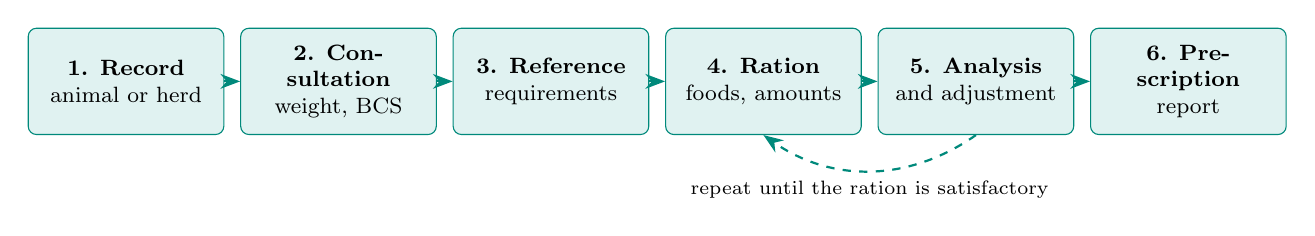
\begin{tikzpicture}[
  etape/.style={rectangle,rounded corners=3pt,draw=vetprimaire,fill=vetfond,
    text width=2.25cm,align=center,minimum height=1.35cm,font=\footnotesize},
  fleche/.style={-{Stealth[length=2.5mm]},thick,vetprimaire}]
  \node[etape] (a) {\textbf{1. Record}\\animal or herd};
  \node[etape,right=0.2cm of a] (b) {\textbf{2. Consultation}\\weight, BCS};
  \node[etape,right=0.2cm of b] (c) {\textbf{3. Reference}\\requirements};
  \node[etape,right=0.2cm of c] (d) {\textbf{4. Ration}\\foods, amounts};
  \node[etape,right=0.2cm of d] (e) {\textbf{5. Analysis}\\and adjustment};
  \node[etape,right=0.2cm of e] (f) {\textbf{6. Prescription}\\report};
  \draw[fleche] (a) -- (b);
  \draw[fleche] (b) -- (c);
  \draw[fleche] (c) -- (d);
  \draw[fleche] (d) -- (e);
  \draw[fleche] (e) -- (f);
  \draw[fleche,dashed] (e.south) to[bend left=35] node[below,font=\scriptsize,text=black]
    {repeat until the ration is satisfactory} (d.south);
\end{tikzpicture}
\caption{The formulation workflow in VetNutri MP.}
\label{fig:demarche}
\end{figure}

\subsection{How to read this guide}

\begin{itemize}
  \item Interface labels are written \ui{like this}, as they appear in the English interface.
  \item The screenshots show the French interface; the buttons and their positions are the
        same in English.
  \item On the screenshots, the markers \rep{1} \rep{2} \rep{3} refer to the explanations that
        follow the figure.
  \item Four kinds of boxes help you understand and check:
\end{itemize}

\begin{aretenir}
The essentials to remember.
\end{aretenir}
\begin{pourquoi}
The nutritional reasoning behind what the application does.
\end{pourquoi}
\begin{verifiez}
The expected result on screen. If you see something else, read the step again.
\end{verifiez}
\begin{attention}
An irreversible action or a common mistake.
\end{attention}

VetNutri MP is a decision-support tool. It replaces neither the clinical examination nor the
veterinarian's judgement; the veterinarian remains responsible for the data entered and the
rations prescribed. Data is stored on your computer and is only sent elsewhere if you export or
share it.

% ================================================================== 2
\section{Installation and first launch}
\label{sec:lancement}

On the very first start, the application database is empty. Three one-off actions make it
ready to use.

\subsection{Install the data}

\begin{enumerate}
  \item Start VetNutri MP. A \ui{Data update} window opens.
  \item Click \ui{Install update}. Installation takes about a minute.
\end{enumerate}

\capture{01_mise_a_jour_donnees.png}{Data installation offered at first launch.}{maj}

\begin{pourquoi}
The built-in data contains the food database, the requirement references and the advice
library. Without it, you could neither choose a reference nor build a ration. The same window
reappears when a new version brings more recent data; \ui{Later} postpones the installation.
\end{pourquoi}

\subsection{Accept the terms of use}

\begin{enumerate}[resume]
  \item At the bottom of the welcome screen, click \ui{Read and accept terms}.
  \item Read the terms, then click \ui{I accept terms}.
\end{enumerate}

\capture{03_cgu.png}{Terms of use.}{cgu}

\subsection{Enter the application}

\begin{enumerate}[resume]
  \item Click \ui{Continue}.
\end{enumerate}

\captureannotee{04_accueil_continuer.png}{Welcome screen, ready to use.}{accueil}{%
  \repere{55}{484}{1}
  \repere{560}{756}{2}
  \repere{560}{816}{3}
  \repere{560}{872}{4}}

\rep{1} Database status: number of foods, references and advice items.
\rep{2} \ui{Continue} opens the application.
\rep{3} \ui{Restore a backup} reloads a backup (section~\ref{sec:sauvegardes}).
\rep{4} \ui{Exam mode} is used for supervised exam sessions.

\begin{verifiez}
The box reads \ui{Complete database}, with more than 11,000 foods. On later launches, simply
click \ui{Continue}.
\end{verifiez}

\begin{aretenir}
The interface language is chosen on this welcome screen (\ui{Language}).
\end{aretenir}

% ================================================================== 3
\section{The main screen}
\label{sec:liste}

The main screen is the list of animals. Everything starts from here.

\captureannotee{05_liste_animaux.png}{The animal list and its controls.}{liste}{%
  \repere{184}{84}{1}
  \repere{528}{84}{2}
  \repere{872}{84}{3}
  \repere{1215}{84}{4}
  \repere{40}{150}{5}
  \repere{1000}{150}{6}
  \repere{1358}{145}{7}
  \repere{1296}{258}{8}
  \repere{1356}{815}{9}
  \repere{1325}{32}{10}}

\begin{tabularx}{\linewidth}{@{}c X@{}}
\rep{1} & \ui{Food list}: browse and edit the food database (section~\ref{sec:aliments}). \\
\rep{2} & \ui{Calculation data}: equations, bibliography, references, advice (section~\ref{sec:donnees}). \\
\rep{3} & \ui{Multi-ration exploration}: calculate rations in series (section~\ref{sec:multiration}). This button only appears when the feature is enabled. \\
\rep{4} & \ui{Quick Import}: import animal records. \\
\rep{5} & Search by ID, name, owner or breed. \\
\rep{6} & Filter by species. \\
\rep{7} & Sorting and advanced filters. \\
\rep{8} & The arrow opens the animal's record; the red bin deletes it. \\
\rep{9} & \ui{+} creates a new record. \\
\rep{10} & Application settings (section~\ref{sec:parametres}). \\
\end{tabularx}

% ================================================================== 4
\section{Worked example: Filou's ration, step by step}
\label{sec:cas}

\begin{tcolorbox}[colback=vetfond,colframe=vetprimaire,boxrule=0.6pt,arc=2pt,
  title=The case,fonttitle=\bfseries]
Filou is a 7-year-old intact male Labrador retriever. He weighs 32~kg and his body condition
score (BCS) is 7/9: he is overweight. The goal is gradual weight loss with a commercial
low-calorie food.

We will create his record, save the consultation, build the ration, correct it using the
analysis, then prepare the prescription.
\end{tcolorbox}

% ------------------------------------------------------------------
\etape{Step 1 — Create the record}{record Filou's identity.}

\begin{enumerate}
  \item In the animal list, click \ui{+} at the bottom right.
  \item Leave \ui{Record: Individual} selected.
  \item Enter the \ui{ID} (for example the clinic's file number), the \ui{Name} and the
        \ui{Owner}.
  \item Choose the \ui{Species} (\emph{Dog}), then enter the \ui{Breed}, the
        \ui{Birth date} and the \ui{Sex}.
  \item Confirm with the tick button at the bottom right.
\end{enumerate}

\captureannotee{06_creation_individu.png}{The form for creating an individual.}{creation-individu}{%
  \repere{545}{152}{1}
  \repere{318}{465}{2}
  \repere{850}{697}{3}
  \repere{318}{833}{4}
  \repere{1290}{856}{5}}

\begin{tabularx}{\linewidth}{@{}c X@{}}
\rep{1} & \ui{Individual} for a single animal, \ui{Herd / group of animals} for a group. \\
\rep{2} & The species: it filters the references and growth curves offered. \\
\rep{3} & The birth date: type it, or use \ui{Select a date} or \ui{Today}. \\
\rep{4} & Sex and reproductive status. \\
\rep{5} & The tick button saves the record. \\
\end{tabularx}

\begin{pourquoi}
The species matters: it filters the references and growth curves on offer. Sex and birth date
are used for the growth curves and to calculate age. For a group of animals, choose
\ui{Herd / group of animals} instead (section~\ref{sec:troupeau}).
\end{pourquoi}

% ------------------------------------------------------------------
\etape{Step 2 — Open the animal's record}{find the working tabs.}

In the list, click the arrow on Filou's row. The record opens on the \ui{Identification} tab.

\captureannotee{08_fiche_identification.png}{The animal's record.}{fiche}{%
  \repere{150}{40}{1}
  \repere{222}{116}{2}
  \repere{222}{172}{3}
  \repere{222}{228}{4}
  \repere{222}{312}{5}
  \repere{222}{396}{6}
  \repere{222}{649}{7}
  \repere{222}{781}{8}
  \repere{1336}{72}{9}}

\begin{tabularx}{\linewidth}{@{}c X@{}}
\rep{1} & Name, species and ID of the open animal. \\
\rep{2} & \ui{Identification}: the information entered in step 1. \\
\rep{3} & \ui{Consultations}: consultation history (step 3). \\
\rep{4} & \ui{Rations}: building and analysing rations (steps 5 to 7). \\
\rep{5} & \ui{Graph} and \ui{Food Graph}: weight monitoring and comparisons (section~\ref{sec:graphiques}). \\
\rep{6} & \ui{Prescription}: documents for the owner (step 8). \\
\rep{7} & \ui{Export animal} and \ui{Share online}: send the record. \\
\rep{8} & \ui{Back} to the animal list. \\
\rep{9} & Edit or delete the record. \\
\end{tabularx}

% ------------------------------------------------------------------
\etape{Step 3 — Enter the consultation}{describe Filou's condition today.}

\begin{enumerate}
  \item Open the \ui{Consultations} tab, then click \ui{+} at the bottom right.
  \item Check the \ui{Date} \rep{1} and enter the \ui{Weight} \rep{2}: 32.
  \item Click the three dots of the \ui{Body condition score} \rep{3} and choose
        \emph{7/9 — Overweight} (figure~\ref{fig:nec}).
  \item Read the ideal weight \ui{Estimation} \rep{5}: 26.67~kg. If you accept it, enter it in
        \ui{Ideal weight (kg)} \rep{4}.
  \item Enter the \ui{Objective} \rep{6}: \emph{gradual weight loss}. If needed, add
        \ui{Keywords} \rep{7} (conditions, context) and an observation.
\end{enumerate}
Do not confirm yet: the reference still has to be chosen (step 4).

\captureannotee{10_consultation_edition.png}{Entering the consultation.}{consultation}{%
  \repere{262}{100}{1}
  \repere{262}{180}{2}
  \repere{1328}{335}{3}
  \repere{262}{464}{4}
  \repere{1104}{447}{5}
  \repere{262}{551}{6}
  \repere{430}{649}{7}
  \repere{1356}{805}{8}}

\rep{8} The tick button saves the consultation (step 4).

\capture{11_consultation_nec.png}{Choosing the body condition score out of 9.}{nec}

\begin{pourquoi}
The ideal weight is the weight on which requirements are calculated. For an overweight animal,
calculating requirements on the current weight would maintain the excess weight.
\begin{itemize}
  \item The \ui{Estimation} is a suggestion calculated from weight and BCS
        (section~\ref{sec:calculs}).
  \item It is only used if you copy it into \ui{Ideal weight (kg)}. Otherwise, calculations
        use the current weight.
\end{itemize}
\end{pourquoi}

% ------------------------------------------------------------------
\etape{Step 4 — Choose the reference}{tell the application which requirements to compare the ration with.}

\begin{enumerate}
  \item Scroll the form down to \ui{Nutritional references}.
  \item In \ui{General reference}, click the three dots: the list of references for the
        species opens.
  \item Type a few letters in the search box \rep{1} if the list is long, then click the
        row you want \rep{3}: here \emph{Adulte >25kg} (adult over 25~kg).
  \item If the animal has a disease to take into account, add it under
        \ui{Complementary references}.
  \item Confirm the consultation with the tick button.
\end{enumerate}

\captureannotee{13_choix_referentiel.png}{Choosing the general reference.}{referentiel}{%
  \repere{418}{263}{1}
  \repere{418}{306}{2}
  \repere{418}{462}{3}}

\rep{2} The number of references matching the search.

\begin{pourquoi}
The reference holds the requirements (minimum, optimum, maximum) of each nutrient for one type
of animal, as well as the energy requirement equation. It is the yardstick the ration is
compared with: a wrong reference gives a wrong analysis, even with a good ration.
The \ui{Energy adjustment coefficients} K1 to K5, further down the form, adjust the energy
requirement (activity, neutering, environment\ldots).
\end{pourquoi}

\begin{attention}
A consultation without a general reference cannot be saved: the application shows
\ui{Missing information}.
\end{attention}

\begin{verifiez}
The consultation appears in the list with its date, the weight and \ui{Rations: 1}.
The application has created a first, empty ration: the ``current ration''.
\end{verifiez}

% ------------------------------------------------------------------
\etape{Step 5 — Build the ration}{put a food in the ration and set its amount.}

\begin{enumerate}
  \item Open the \ui{Rations} tab. In the \ui{Ration foods} panel, click \ui{+}.
  \item Type a name, a brand or an ingredient \rep{1}: here \emph{satiety}. Narrow down if
        needed with the filters \rep{2} (type, indications, species, database).
  \item Click a food in the list \rep{3}: its details appear on the right \rep{4} (brand,
        species, indications, ingredients, composition). Check that it is a dog food.
  \item Click the round \ui{+} button \rep{5}: the food is added with an amount of 100~g. The
        \ui{+R} button \rep{6} adds it to a new ration instead.
  \item Go back to the ration with the arrow at the top left.
\end{enumerate}

\captureannotee{14_ajout_aliment.png}{Searching for and adding a food.}{ajout-aliment}{%
  \repere{270}{122}{1}
  \repere{270}{212}{2}
  \repere{258}{605}{3}
  \repere{940}{124}{4}
  \repere{1295}{768}{5}
  \repere{1295}{848}{6}}

To set the amount, click the pencil on the food's row, enter the amount in grams (here 380) and
confirm with \ui{OK}.

% ------------------------------------------------------------------
\etape{Step 6 — Read the analysis}{find out whether the ration meets Filou's requirements.}

With 380~g of the food, the \ui{Rations} tab looks like this.

\captureannotee{15_ration_avant_ajustement.png}{Analysis of the 380~g ration.}{ration-avant}{%
  \repere{252}{103}{1}
  \repere{636}{103}{2}
  \repere{1020}{101}{3}
  \repere{252}{212}{4}
  \repere{252}{576}{5}
  \repere{836}{212}{6}
  \repere{1180}{185}{7}
  \repere{836}{248}{8}}

\begin{tabularx}{\linewidth}{@{}c X@{}}
\rep{1} & \ui{Metabolic values}: weight, ideal weight, metabolic weight, standard energy
          requirement (BEE) and energy requirement (BE). \\
\rep{2} & \ui{Coefficients} K1 to K5 and the adjustment coefficient. The pencil edits them. \\
\rep{3} & \ui{Energy balance}: energy supplied, requirement coverage, observed K and
          calculated K. \textbf{This is the first figure to look at.} \\
\rep{4} & The consultation's rations. \\
\rep{5} & The foods of the selected ration and the adjustment tools. \\
\rep{6} & \ui{INTAKES}: each nutrient, expressed in the reference's unit (here ``per
          1000 kcal''). \\
\rep{7} & Expression unit, nutrients shown, PDF export, card or chart view. \\
\rep{8} & Nutrients by family. A warning icon flags a deviation from the reference. \\
\end{tabularx}

\subsubsection{Interpreting the result}

Energy coverage is only 56~\%: 380~g supply 971~kcal/day for a requirement of
1749~kcal/day. Almost every nutrient is flagged as deficient.

\begin{pourquoi}
Intakes are related to the animal's energy requirement, not to the energy of the ration
(section~\ref{sec:calculs}). As long as the ration does not meet the energy requirement, every
intake looks low. \textbf{So always correct energy first}, then look at the other nutrients.
\end{pourquoi}

% ------------------------------------------------------------------
\etape{Step 7 — Adjust the ration}{reach an energy coverage close to 100~\%.}

\subsubsection{Quick adjustment}

In the \ui{Ration foods} panel, click the \ui{Quick multi-nutrient adjustment} icon (the scales,
to the left of the book and the \ui{+}). The amounts are recalculated to meet the energy
requirement.

\captureannotee{17_ration_apres_ajustement.png}{The same ration after quick adjustment.}{ration-apres}{%
  \repere{1160}{150}{1}
  \repere{252}{646}{2}
  \repere{1000}{406}{3}}

\begin{verifiez}
\rep{1} Coverage rises to 99~\% and the observed K to 0.99. \rep{2} The amount rises to
675~g. \rep{3} The deficiency warnings disappear; small red arrows now flag a few intakes above
the optimum maximum (calcium, phosphorus, vitamin~A).
\end{verifiez}

\begin{pourquoi}
Exceeding the optimum is not necessarily a problem: hover over the icon to read the threshold
involved and judge it clinically. For weight loss, energy is set through the ideal weight and
the K coefficients, not by feeding less than the calculated ration: otherwise the other
nutrients become insufficient.
\end{pourquoi}

\subsubsection{Multi-nutrient adjustment}

The neighbouring icon opens the full tool, useful when the ration combines several foods.

\captureannotee{16_ajustement_multinutriments.png}{Multi-nutrient adjustment.}{ajustement}{%
  \repere{268}{147}{1}
  \repere{268}{320}{2}
  \repere{1385}{240}{3}
  \repere{1220}{448}{4}
  \repere{268}{552}{5}
  \repere{268}{719}{6}}

\begin{tabularx}{\linewidth}{@{}c X@{}}
\rep{1} & Quick actions: lock or unlock all amounts, automatic adjustment, reset. \\
\rep{2} & For each food, the \ui{Target nutrient} it must cover. \\
\rep{3} & The padlock freezes a food's amount. \\
\rep{4} & The target level for each target nutrient (minimum, optimum\ldots). \\
\rep{5} & The share of the energy requirement covered by complete foods, when the ration
          combines a complete food and supplements. \\
\rep{6} & \ui{Preview} without changing anything, \ui{Adjust}, \ui{Equal quantity (Sanalio)}, or
          \ui{Constraint-based adjustment (min/max)}, which tries to respect all the reference's
          bounds at once. \\
\end{tabularx}

\subsubsection{Viewing the ration as a chart}

The \ui{Cards} / \ui{Bullet} switch of the \ui{INTAKES} panel shows the composition of the
ration, where the energy comes from and, for each nutrient, a bar compared with the
reference's thresholds. \ui{Click for more details} opens the detail of a nutrient.

\captureannotee{18_analyse_graphique.png}{Ration analysis in chart view.}{analyse-graphique}{%
  \repere{1380}{240}{1}
  \repere{862}{256}{2}
  \repere{1135}{256}{3}
  \repere{1030}{700}{4}
  \repere{1190}{595}{5}}

\begin{tabularx}{\linewidth}{@{}c X@{}}
\rep{1} & The \ui{Cards} / \ui{Bullet} switch toggles between the card view and this chart view. \\
\rep{2} & \ui{Composition}: the share of each constituent in the ration, by mass. \\
\rep{3} & \ui{Energy Origin}: the share of energy supplied by protein, fat and NFE. \\
\rep{4} & For each nutrient, a bar places the intake against the reference's thresholds. \\
\rep{5} & \ui{Click for more details} opens the nutrient's detail. \\
\end{tabularx}

% ------------------------------------------------------------------
\etape{Step 8 — Prepare the prescription}{give the owner a clear ration and advice.}

\begin{enumerate}
  \item Open the \ui{Prescription} tab.
  \item Tick the ration or rations to prescribe \rep{1}.
  \item Add advice from the library or write a \ui{New section} \rep{2}.
  \item Fill in the report \rep{3}: history, clinical examination, key nutritional factor,
        additional text.
  \item Use the buttons at the bottom \rep{4}: \ui{Copy report} (to paste into your practice
        software), \ui{Preview report}, \ui{Preview prescription}.
\end{enumerate}

\captureannotee{21_ordonnance.png}{Preparing the prescription and the report.}{ordonnance}{%
  \repere{278}{160}{1}
  \repere{268}{325}{2}
  \repere{830}{175}{3}
  \repere{585}{861}{4}}

\begin{aretenir}
The practitioner's details printed on the prescription are entered once and for all in
\ui{Settings} > \ui{Preferences} (section~\ref{sec:parametres}).
\end{aretenir}

% ------------------------------------------------------------------
\subsection{Summary of the case}

\begin{tabularx}{\linewidth}{@{}l l X@{}}
\toprule
\textbf{Step} & \textbf{Where} & \textbf{Result for Filou} \\
\midrule
1. Record & List, \ui{+} & male Labrador, born in 2019 \\
3. Consultation & \ui{Consultations} & 32 kg, BCS 7/9, estimated ideal weight 26.67 kg \\
4. Reference & consultation form & \emph{Adulte >25kg} \\
5. Ration & \ui{Rations}, \ui{+} & a low-calorie food, 380 g \\
6. Analysis & \ui{Rations} & 56 \% coverage, apparent deficiencies \\
7. Adjustment & quick adjustment & 675 g, 99 \% coverage \\
8. Prescription & \ui{Prescription} & ration ticked, report, printing \\
\bottomrule
\end{tabularx}

\begin{aretenir}
At a follow-up visit, do not edit the previous consultation: create a new one, or duplicate the
previous one with the copy icon. The weight and ration history then stays readable in the
graphs.
\end{aretenir}

% ================================================================== 5
\section{Understanding the calculations}
\label{sec:calculs}

This section explains the figures shown in the \ui{Rations} tab, using Filou's values.

\subsection{The calculation weight}

Requirements are calculated on the \textbf{ideal weight} if it has been entered, otherwise on the
current weight. The estimate offered in the consultation assumes that each BCS point above 5
corresponds to 10~\% excess weight:
\[
  \text{estimated ideal weight} = \frac{\text{weight} \times 100}{100 + (\text{BCS} - 5) \times 10}
  \qquad\text{Filou: } \frac{32 \times 100}{120} = 26.67\ \text{kg}
\]

\subsection{From weight to energy requirement}

\begin{enumerate}
  \item The \textbf{metabolic weight} reflects the fact that requirements do not increase in
        proportion to weight:
        \[ W_{\text{met}} = W^{0.75} \qquad\text{Filou: } 32^{0.75} = 13.45\ \text{kg}^{0.75} \]
  \item The \textbf{standard energy requirement} (BEE) applies the reference's equation. For
        the reference in the example:
        \[ \text{BEE} = 130 \times W^{0.75} = 130 \times 13.45 = 1749\ \text{kcal/day} \]
  \item The \textbf{calculated K} is the product of coefficients K1 to K5 and of the adjustment
        coefficient. The \textbf{energy requirement} (BE) follows from it, increased where
        relevant by the energy required by disease references:
        \[ \text{BE} = \text{BEE} \times K \;(+\ \text{energy from complementary references}) \]
\end{enumerate}

\begin{aretenir}
In the example, the ideal weight was not copied over: calculations use 32~kg. With 26.67~kg,
the BEE would drop to $130 \times 26.67^{0.75} \approx 1525$~kcal/day.
\end{aretenir}

\subsection{Energy supplied by foods}

A food's energy comes from, in this order:
\begin{enumerate}
  \item the value entered for the species in the food's record;
  \item otherwise the reference's energy density equation: for dogs, the equation for
        commercial foods (complete or complementary foods), otherwise the Atwater equation (raw
        foods).
\end{enumerate}
The dog commercial-food equation takes fibre into account:
\[
  \text{ME (kcal/100 g)} = \bigl(5.7\,P + 9.4\,L + 4.1\,(\text{NFE} + C)\bigr)
  \times \frac{91.2 - 1.43\,\dfrac{100\,C}{100 - H}}{100} - 1.04\,P
\]
where $P$ is protein, $L$ fat, $C$ crude fibre and $H$ moisture, in \%.
\begin{itemize}
  \item If crude fibre is not entered, \textbf{total dietary fibre} is used instead.
  \item If nitrogen-free extract (NFE) is not entered, it is calculated:
        $100 - P - H - C - \text{ash} - L$. The estimated crude fibre is subtracted, so that
        fibre is not counted twice.
\end{itemize}
Example: a puppy milk with 33~\% protein, 39~\% fat, 19.5~\% NFE, 3~\% moisture and 0.5~\%
total fibre supplies 541.7~kcal/100~g, i.e.\ 1083~kcal for 200~g.

\subsection{The energy balance}

\[
  \text{Coverage} = \frac{\text{energy supplied}}{\text{BE}}
  \qquad\qquad
  K_{\text{observed}} = \frac{\text{energy supplied}}{\text{BEE}}
\]
With 675~g: $1725 / 1749 = 99~\%$ and $K_{\text{observed}} = 0.99$. The observed K shows which
coefficient the ration actually applies; compare it with the calculated K.

\subsection{Intakes}

Intakes are expressed in the reference's unit. In ``per 1000 kcal'', the daily intake is related
to the \textbf{standard energy requirement} (BEE), not to the energy of the ration:
\[
  \text{intake (g/1000 kcal)} = \frac{\text{daily intake (g/day)}}{\text{BEE (kcal/day)}} \times 1000
\]
Since the reference's thresholds are expressed the same way, the comparison amounts to
comparing the daily intake with the animal's daily requirement. Filou, with 675~g of a food
containing 30~\% protein: $202.5 / 1749 \times 1000 = 116$~g/1000~kcal.

\begin{aretenir}
If the ration only covers half of the energy requirement, every intake is half of what it would
be with the right amount. Hence the rule: \textbf{energy first}.
\end{aretenir}

\subsection{Warnings}

\begin{tabularx}{\linewidth}{@{}>{\raggedright\arraybackslash}p{6.2cm} X@{}}
\toprule
\textbf{Message (on hovering over the icon)} & \textbf{Meaning} \\
\midrule
Deficiency: intake below the minimum & below the reference's minimum threshold. \\
Deficiency: intake below the optimal minimum & above the minimum, but below the optimum. \\
Excess: intake above the optimal maximum & above the optimum (red arrow). \\
Incomplete information & the composition of at least one food does not give this nutrient:
the actual intake may be higher. \\
\bottomrule
\end{tabularx}

The \ui{Analyses and Ratios} section gives the K/Na, Ca/P, omega-6/omega-3 and Zn/Cu ratios,
calculated on the whole ration and rounded to two decimals (Ca/P = 1.1 / 0.8 = 1.38).

% ================================================================== 6
\section{Going further with rations}

\subsection{Several rations in one consultation}

A consultation can hold the owner's current ration and one or more proposals, to compare them.
\begin{itemize}
  \item \ui{+} in the \ui{Consultation rations} panel adds a ration; the icon next to it reuses a
        ration from a previous consultation.
  \item On each ration: add a step to the progressive plan (food transition), duplicate, edit,
        delete.
  \item In \ui{Ration foods}: save the ration as a recipe, copy it, open the saved recipes.
\end{itemize}

\subsection{Monitoring graphs}
\label{sec:graphiques}

The \ui{Graph} tab offers four views: \ui{Weight evolution}, \ui{Energy distribution},
\ui{Energy density of rations} and \ui{Ration nutrients}.

\captureannotee{19_graphique_poids.png}{Weight evolution and reference curves.}{graphique-poids}{%
  \repere{440}{176}{1}
  \repere{900}{176}{2}
  \repere{1095}{176}{3}
  \repere{895}{506}{4}
  \repere{265}{830}{5}
  \repere{745}{862}{6}
  \repere{1245}{857}{7}}

\begin{tabularx}{\linewidth}{@{}c X@{}}
\rep{1} & The suggested reference curve (sex and weight class); click to choose another one. \\
\rep{2} & Enlarging the growth curves and exporting them to PDF. \\
\rep{3} & Show or hide the reference curves. \\
\rep{4} & Each weighing, plotted against age. \\
\rep{5} & The animal's \ui{Weight history}. \\
\rep{6} & The weight-loss target: minimum and maximum loss in \% per week, target weight. \\
\rep{7} & The \ui{+} button adds a weighing. \\
\end{tabularx}

The weight view plots each weighing against age. Below the graph, the \ui{Weight history} lets
you add a weighing and set a weight-loss target (minimum and maximum loss in \% per week).

\begin{pourquoi}
The reference curve offered by default matches the animal's sex and weight class. That class is
set, in this order:
\begin{enumerate}
  \item by the expected adult weight, for a puppy (variable AW of the consultation);
  \item otherwise by the ideal weight, entered or estimated from the BCS;
  \item otherwise by the latest weight.
\end{enumerate}
An overweight animal is therefore not placed in too high a class. The button above the graph
lets you choose another curve.
\end{pourquoi}

In the ration views, each ration has a number, repeated in the legend below the graph: 1,
2\ldots{} for the rations of the first consultation, 101, 102\ldots{} for the next one. Two
options control the display:
\begin{itemize}
  \item \ui{Current consultation only} limits the graph to
        the consultation on display;
  \item \ui{Area of possibilities and sums} outlines the
        rations of each consultation (orange for current rations, blue for proposals) and adds
        their mean weighted by the coefficients, marked \textbf{$\Sigma$}. Ration numbers do
        not change.
\end{itemize}

The \ui{Food Graph} tab compares foods with each other: add them with \ui{+} in the list on the
left, then click \ui{View graphic analysis}.

\captureannotee{20_graphique_aliments.png}{Selecting foods to compare.}{graphique-aliments}{%
  \repere{268}{57}{1}
  \repere{495}{272}{2}
  \repere{752}{324}{3}
  \repere{1112}{272}{4}
  \repere{1125}{860}{5}}

\begin{tabularx}{\linewidth}{@{}c X@{}}
\rep{1} & Search and filters (type, species, database, indications). \\
\rep{2} & The foods found; the \ui{+} on a row adds the food to the comparison. \\
\rep{3} & \ui{Add all} and \ui{Remove all}. \\
\rep{4} & The selected foods. \\
\rep{5} & \ui{View graphic analysis} opens the comparison charts. \\
\end{tabularx}

\subsection{Sending a record}

From the record's left-hand menu:
\begin{itemize}
  \item \ui{Export animal} saves the complete record (consultations, rations, foods used) to a
        file that can be imported on another computer;
  \item \ui{Share online} sends the record through an online service.
\end{itemize}

% ================================================================== 7
\section{Special cases}

\subsection{A herd}
\label{sec:troupeau}

\textbf{When to use it?} To work out a ration for a whole facility or group of animals: a
kennel, a cattery, a batch of farm animals.

When creating the record, choose \ui{Herd / group of animals}. A herd has no species, breed or
sex of its own: it is described by groups of individuals (name, number, mean weight, species,
breed, sex). It can mix several species; each group's reference and K are chosen in each
consultation.

\captureannotee{07_creation_troupeau.png}{Creating a herd of twelve individuals.}{creation-troupeau}{%
  \repere{545}{152}{1}
  \repere{345}{441}{2}
  \repere{1105}{448}{3}
  \repere{474}{612}{4}
  \repere{305}{636}{5}
  \repere{1290}{856}{6}}

\begin{tabularx}{\linewidth}{@{}c X@{}}
\rep{1} & \ui{Herd / group of animals} is selected. \\
\rep{2} & The herd's total number of animals, the sum of the groups. \\
\rep{3} & For each group: its name, the number of animals and their mean weight; the cross removes the group. \\
\rep{4} & The group's species, breed and sex. \\
\rep{5} & \ui{Add a group of animals}; a new group takes the species of the previous one. \\
\rep{6} & The tick button saves the herd. \\
\end{tabularx}

\subsubsection{The consultation}

The \ui{Herd status} replaces the individual's weight, BCS, reference and K. For each group,
enter the number of animals and their mean weight on the date of the consultation, the mean body
condition score, the reference (for the group's species) and the group's K, together with any
variables of the reference's equations. The requirement of one animal is the reference's
standard requirement multiplied by the group's K.

\subsubsection{The ration and its analysis}

A herd's rations are entered as daily amounts for the whole herd. The \ui{Rations} tab shows the
herd panel above the rations.

\captureannotee{37_troupeau_rations.png}{The ration of a herd of twelve dogs in two groups.}{troupeau-rations}{%
  \repere{1190}{128}{1}
  \repere{675}{145}{2}
  \repere{250}{168}{3}
  \repere{252}{275}{4}
  \repere{840}{398}{5}}

\begin{tabularx}{\linewidth}{@{}c X@{}}
\rep{1} & \ui{Adjust the ration to the herd's energy requirement} multiplies every amount by the
          factor shown (here $\times 0.988$) so that the energy supplied equals the herd's
          requirement. \\
\rep{2} & What is analysed: \ui{Whole herd}, or one group (its name and number of animals). \\
\rep{3} & The herd's daily ration, the herd's requirement, the energy supplied and the coverage
          (green from 90 to 110~\%, orange up to 80 and 120~\%, red beyond). \\
\rep{4} & One row per group: share of the ration, requirement and energy of one animal,
          coverage, number of out-of-range nutrients and ration of one animal. \\
\rep{5} & \ui{Whole-herd intakes}, nutrient by nutrient. \\
\end{tabularx}

\begin{pourquoi}
The herd ration is shared between the groups in proportion to their energy requirement: one
animal of group $i$ receives
\[
  \text{amount} \times \frac{B_i}{\sum_j n_j\,B_j}
\]
where $n_j$ is the number of animals in group $j$ and $B_j$ the energy requirement of one of
them. In the example, a 25~kg adult receives 271.6~g and a 20~kg senior (K = 0.9) 206.8~g.
\end{pourquoi}

\textbf{Analysing a group.} Click a group's row (or its chip): the ration shown becomes that of
one animal of the group, analysed like a single animal's ration, with the group's weight,
reference and K. This ration is read-only; click the row again, or \ui{Whole herd}, to return
to the herd ration and edit it.

\textbf{The whole herd.} The \ui{Whole-herd intakes} table compares the total daily intake with
the sum of the animals' requirements (number $\times$ requirement of one animal, group by group),
for each nutrient: energy first, then out-of-range nutrients, then the others in alphabetical
order. \ui{Only out-of-range nutrients} shortens the list. An asterisk marks an incomplete
value: the composition of at least one food does not give this nutrient.

\begin{attention}
A compliant total can hide a deficiency in one group: an over-fed group makes up, in the total,
for a group that falls short. Always check the last column, \ui{Out-of-range groups}, and the
number of deviations of each group in the upper table.
\end{attention}

\subsection{Multi-ration exploration}
\label{sec:multiration}

\textbf{When to use it?} To prepare standard rations, for example for a whole range of weights,
rather than a ration for one specific animal.

First enable it in \ui{Settings} > \ui{Administration} > \ui{Enable multi-ration analysis}; the \ui{Multi-ration exploration} button then appears in the animal list.

\captureannotee{28_multiration.png}{Setting up a multi-ration exploration.}{multiration}{%
  \repere{455}{150}{1}
  \repere{440}{191}{2}
  \repere{440}{250}{3}
  \repere{440}{343}{4}
  \repere{440}{724}{5}
  \repere{440}{815}{6}}

\begin{tabularx}{\linewidth}{@{}c X@{}}
\rep{1} & The number of scenarios to calculate and what still blocks the calculation. \\
\rep{2} & \ui{Calculate all rations}, active once the configuration is complete. \\
\rep{3} & The tabs: \ui{Animals}, \ui{Ingredients}, \ui{Options}, \ui{Saved}. \\
\rep{4} & The species and the general references to combine. \\
\rep{5} & The weight grid (from, to, step). \\
\rep{6} & The K coefficient grid (from, to, step). \\
\end{tabularx}

\begin{enumerate}
  \item Choose the species and tick one or more general references.
  \item Define the grid: weight (from, to, step) and K coefficient (from, to, step). The number
        of scenarios is shown.
  \item In the \ui{Ingredients} tab, build the lists of foods supplying protein, fibre,
        calcium, omega-6, salt and energy. The adjustment follows this order.
  \item Click \ui{Calculate all rations}. Clicking a cell of the
        map shows its rations, which can be opened in the usual analysis to edit and export
        them.
\end{enumerate}
The \ui{Saved} tab keeps named configurations; results are recalculated each
time they are opened.

% ================================================================== 8
\section{Managing data}

\subsection{The food database}
\label{sec:aliments}

\ui{Food list} (main screen) shows the whole database, with the same filters as the food search
of a ration. The pencil edits a food, the bin deletes it, \ui{+} creates one.

\captureannotee{22_liste_aliments.png}{Food list.}{aliments}{%
  \repere{690}{121}{1}
  \repere{700}{196}{2}
  \repere{72}{295}{3}
  \repere{780}{280}{4}
  \repere{1300}{856}{5}}

\begin{tabularx}{\linewidth}{@{}c X@{}}
\rep{1} & Search by name, brand or ingredient. \\
\rep{2} & Filters: type, indications, species, database. \\
\rep{3} & The pencil edits the food, the bin deletes it. \\
\rep{4} & Food type, species and indications. \\
\rep{5} & \ui{+} creates a food. \\
\end{tabularx}

A food record has three tabs: \ui{General information} (name, brand, range, database, price,
packaging, type), \ui{Nutritional Composition} and \ui{Bibliography}. Save with \ui{Save}.

\captureannotee{23_aliment_edition.png}{Editing a food.}{aliment-edition}{%
  \repere{615}{104}{1}
  \repere{480}{169}{2}
  \repere{1385}{500}{3}
  \repere{1385}{880}{4}}

\begin{tabularx}{\linewidth}{@{}c X@{}}
\rep{1} & \ui{Save} records the changes. \\
\rep{2} & The three tabs: \ui{General information}, \ui{Nutritional Composition}, \ui{Bibliography}. \\
\rep{3} & The food's source database. \\
\rep{4} & The food type: complete or complementary (energy from the commercial-food equation), otherwise raw food (Atwater equation), see section~\ref{sec:calculs}. \\
\end{tabularx}

\begin{aretenir}
An incomplete composition produces ``Incomplete information'' warnings in the analysis. For a
food you create, enter at least energy, macronutrients, calcium and phosphorus.
\end{aretenir}

\subsection{Calculation data}
\label{sec:donnees}

The \ui{Calculation data} button gives access to the elements the calculations rely on. They
ship with the application. Edit them with care: any change alters the analyses of every
consultation that uses them.

\begin{tabularx}{\linewidth}{@{}l X@{}}
\toprule
\textbf{Tab} & \textbf{Content} \\
\midrule
\ui{Equations} & formulas for energy requirement, metabolic weight and energy density (for
example \texttt{130*BW\^{}0.75}) \\
\ui{Bibliography} & references supporting the requirement references and food values \\
\ui{Calculation systems} & the requirement references: by species, life stage or disease \\
\ui{Custom advice} & advice library reused in the prescription \\
\bottomrule
\end{tabularx}

\captureannotee{26_referentiels.png}{Nutritional references (Calculation systems tab).}{referentiels}{%
  \repere{700}{56}{1}
  \repere{650}{156}{2}
  \repere{190}{257}{3}
  \repere{275}{489}{4}
  \repere{1222}{274}{5}
  \repere{1300}{856}{6}}

\begin{tabularx}{\linewidth}{@{}c X@{}}
\rep{1} & The four tabs of the calculation data. \\
\rep{2} & Searching for a reference. \\
\rep{3} & Name, species and physiological stage of the reference. \\
\rep{4} & A red line marks a disease reference, to be added as a complementary reference. \\
\rep{5} & Edit, duplicate or delete the reference. \\
\rep{6} & \ui{+} creates a reference. \\
\end{tabularx}
\capture{24_equations.png}{Equations.}{equations}
\capture{25_bibliographie.png}{Bibliography.}{bibliographie}
\capture{27_conseils.png}{The advice library.}{conseils}

% ================================================================== 9
\section{Settings}
\label{sec:parametres}

The gear icon on the main screen opens the settings, in six tabs.

\begin{tabularx}{\linewidth}{@{}l X@{}}
\toprule
\textbf{Tab} & \textbf{Purpose} \\
\midrule
\ui{Interface} & interface size (50 to 200~\%); access to \ui{Cross analysis} \\
\ui{Preferences} & practitioner's details for the prescription; unit used to express
requirements, by species \\
\ui{Import/Export} & data exchange (animals, foods, recipes, equations, references, advice) \\
\ui{Excel} & export and import of foods as Excel-compatible CSV \\
\ui{Recipes} & recipes saved from rations \\
\ui{Administration} & multi-ration, re-import of the initial data, backups, VetNutri~2 import,
maintenance \\
\bottomrule
\end{tabularx}

\subsection{Preferences: to do right after installation}

Enter your details (name, registration number, address, phone, e-mail), printed on the
prescription, then click \ui{Save}. The \ui{Requirement expression by species} section sets the unit in which requirements are
expressed (for example ``per 1000 kcal'').

\captureannotee{30_param_preferences.png}{Preferences.}{param-preferences}{%
  \repere{700}{58}{1}
  \repere{290}{145}{2}
  \repere{190}{645}{3}
  \repere{395}{713}{4}
  \repere{1300}{812}{5}}

\begin{tabularx}{\linewidth}{@{}c X@{}}
\rep{1} & The six settings tabs. \\
\rep{2} & The practitioner's details, printed on the prescription. \\
\rep{3} & \ui{Save} the details. \\
\rep{4} & \ui{Requirement expression by species}: the unit in which requirements are shown. \\
\rep{5} & Click a species to change its unit (for example ``per 1000 kcal''). \\
\end{tabularx}

\subsection{Interface}

\capture{29_param_interface.png}{Interface size.}{param-interface}

\subsection{Import, export and Excel}

The \ui{Import/Export} tab exports and imports data in API format, with advanced selection, and
imports foods, animals or nutritional references (\texttt{.vbnr.json}).

In a references file, each requirement states its unit: per Mcal (per 1000 kcal), per kg of body
weight, per kg of metabolic weight, as an absolute value or as a ratio. A requirement whose unit
is not recognised (for example ``DM'') is not imported: it is listed in the import report, so
that you can correct the file.

\capture{31_param_import_export.png}{Data import and export.}{param-import}

The \ui{Excel} tab exports and imports foods as CSV: semicolon separator, UTF-8 encoding, one
header row, one column per nutrient with the unit in the header. A preview lets you check the
data before confirming the import.

\capture{32_param_excel.png}{Excel export and import of foods.}{param-excel}

\subsection{Recipes}

\capture{33_param_recettes.png}{Saved recipes.}{param-recettes}

\subsection{Administration}

\captureannotee{34_param_administration.png}{Database administration.}{param-admin}{%
  \repere{1285}{272}{1}
  \repere{40}{338}{2}
  \repere{40}{402}{3}
  \repere{40}{466}{4}
  \repere{40}{530}{5}
  \repere{40}{603}{6}}

\begin{tabularx}{\linewidth}{@{}c X@{}}
\rep{1} & \ui{Enable multi-ration analysis} shows the \ui{Multi-ration exploration} button in the animal list. \\
\rep{2} & Rerun the automatic import of the initial data (foods, references, advice). \\
\rep{3} & \ui{Manage backups} (section~\ref{sec:sauvegardes}). \\
\rep{4} & Import the data of a VetNutri~2 installation. \\
\rep{5} & Add the same bibliographic reference to many foods. \\
\rep{6} & Irreversible actions: clearing a database. \\
\end{tabularx}

\begin{attention}
The red \ui{Clear \ldots{} database} buttons permanently delete the foods, animals, references,
equations or bibliographies. Make a backup before using them.
\end{attention}

\subsection{Backups}
\label{sec:sauvegardes}

\ui{Administration} > \ui{Manage backups} lists the backups with their date, content and size.
\ui{New backup} creates one; on each row, one icon restores it and
another deletes it.

\captureannotee{35_sauvegardes.png}{Managing backups.}{sauvegardes}{%
  \repere{1140}{40}{1}
  \repere{320}{121}{2}
  \repere{700}{176}{3}
  \repere{1270}{120}{4}
  \repere{1375}{120}{5}}

\begin{tabularx}{\linewidth}{@{}c X@{}}
\rep{1} & \ui{New backup}. \\
\rep{2} & The backup's date and file. \\
\rep{3} & Its content: animals, foods, equations, advice, and its size. \\
\rep{4} & Restore this backup: its data is merged with the current data, after an automatic backup is made first. \\
\rep{5} & Delete the backup. \\
\end{tabularx}

\begin{aretenir}
Make a backup before any major operation: bulk import, clearing a database, changing computer.
From time to time, copy a backup off the computer.
\end{aretenir}

\subsection{Cross analysis}
\label{sec:analyses-croisees}

\textbf{When to use it?} To compare many consultations: tutorials, case series, exams.

Filter by species, keywords, exam ID or exercise ID, select the consultations, then open the
analysis or the grading.

\capture{36_analyses_croisees.png}{Cross analysis.}{analyses-croisees}

% ================================================================== Appendices
\appendix

\section{Frequently asked questions}

\begin{description}[style=nextline,leftmargin=0pt,itemsep=6pt]
  \item[I cannot save the consultation.]
    The \ui{General reference} is missing. Choose a reference in the \ui{Nutritional
    references} section of the form.
  \item[No reference appears in the list.]
    Check the animal's species: only references for its species are offered. Also check that
    the data has been installed (welcome screen).
  \item[Every nutrient is deficient.]
    Look at the energy coverage: if it is far from 100~\%, adjust the amount first
    (section~\ref{sec:calculs}).
  \item[The energy requirement looks too high for an overweight animal.]
    Calculations use the current weight as long as the ideal weight is not entered. Copy the
    estimate, or your own value, into \ui{Ideal weight (kg)}.
  \item[The growth curve does not match my puppy.]
    Enter its expected adult weight (variable AW) in the consultation, or choose another curve
    with the button above the graph.
  \item[The multi-ration exploration button does not appear.]
    Enable it in \ui{Settings} > \ui{Administration}.
  \item[The energy of a high-fibre food looks low.]
    When crude fibre is not entered, total dietary fibre, often much higher, is used in its
    place in the equation (section~\ref{sec:calculs}). Enter the crude fibre in the food's
    record if you know it.
  \item[A food is missing from the database.]
    Create it from the \ui{Food list}, or directly from the food search of a ration (\ui{+} at
    the top right).
\end{description}

\section{Glossary}

\begin{tabularx}{\linewidth}{@{}l X@{}}
\toprule
\textbf{Term} & \textbf{Definition} \\
\midrule
BCS & Body condition score, from 1 (very thin) to 9 (very obese); 4 and 5 are ideal. \\
BE & The animal's energy requirement: BEE × K, plus energy related to diseases. \\
BEE & Standard energy requirement, calculated by the reference's equation (kcal/day). \\
Coverage & Share of the BE supplied by the ration (\%). \\
Crude fibre & Fibre fraction used by the energy equation; total dietary fibre if missing. \\
Current ration & First ration of a consultation, often what the animal already eats. \\
Herd & Record describing a group of animals by groups of individuals. \\
Ideal weight & Weight on which requirements are calculated; the current weight if missing. \\
K, K1 to K5 & Coefficients that adjust the energy requirement (activity, neutering\ldots). \\
Metabolic weight & Weight raised to the power 0.75 (kg$^{0.75}$). \\
NFE & Nitrogen-free extract (digestible carbohydrates), in \%; calculated by difference if
missing. \\
Observed K & Energy supplied divided by the BEE: the coefficient actually applied. \\
Reference & Set of requirements (minimum, optimum, maximum) for one type of animal. \\
\bottomrule
\end{tabularx}

\section{Quick reference: a consultation in ten moves}

\begin{enumerate}
  \item Animal list: \ui{+}, or the arrow of an existing animal.
  \item \ui{Consultations}: \ui{+}, or copy the previous consultation.
  \item Weight and BCS.
  \item Ideal weight: copy the estimate or enter your own value.
  \item General reference, plus complementary ones for a disease; confirm.
  \item \ui{Rations}: \ui{+} in \ui{Ration foods}, search, add.
  \item Read the energy balance.
  \item Quick adjustment, or multi-nutrient adjustment.
  \item Review the warnings nutrient by nutrient.
  \item \ui{Prescription}: tick the ration, add advice and report, print.
\end{enumerate}

\end{document}
